\chapter{State of the art}

\section{Intraoperative ultrasound}
Ultrasound imaging works by the \textit{pulse-echo} principle. A short
ultrasound-pulse is emitted from a transducer. Then the soundwaves get
transmitted and reflected differently by different tissues. The reflected
soundwaves travel back into the transducer and get converted into an electrical
signal. After post-processing these signals become ultrasound images. Basically
the ultrasound measures the mechanical properties of the tissue. The tissues
have different acoustic impedance, which is the product of tissue density and
ultrasound speed in travelling through the tissue. The resolution of the
ultrasound images depends on the frequency of the ultrasound waves. High
frequencies lead to high resolutions but low depth into the tissue because the
absorption of the sound energy increases with frequency too. Therefore the
useability to see deep structures is limited \cite{torzilli2014ultrasound}. In
liver surgeries the ultrasound is used for intraoperative planning and
navigation inside the liver. Figure \ref{fig:liverUS} shows an example of an
ultrasound image of the liver and its corresponding position in the 3D liver
model. The surgeon can find the tumors inside the liver by using the ultrasound.
Registration methods based on 3D ultrasound reconstructed liver vessels also
exist but are not used a lot yet \cite{lange2003vessel}.

\begin{figure}[H]
  \centering
 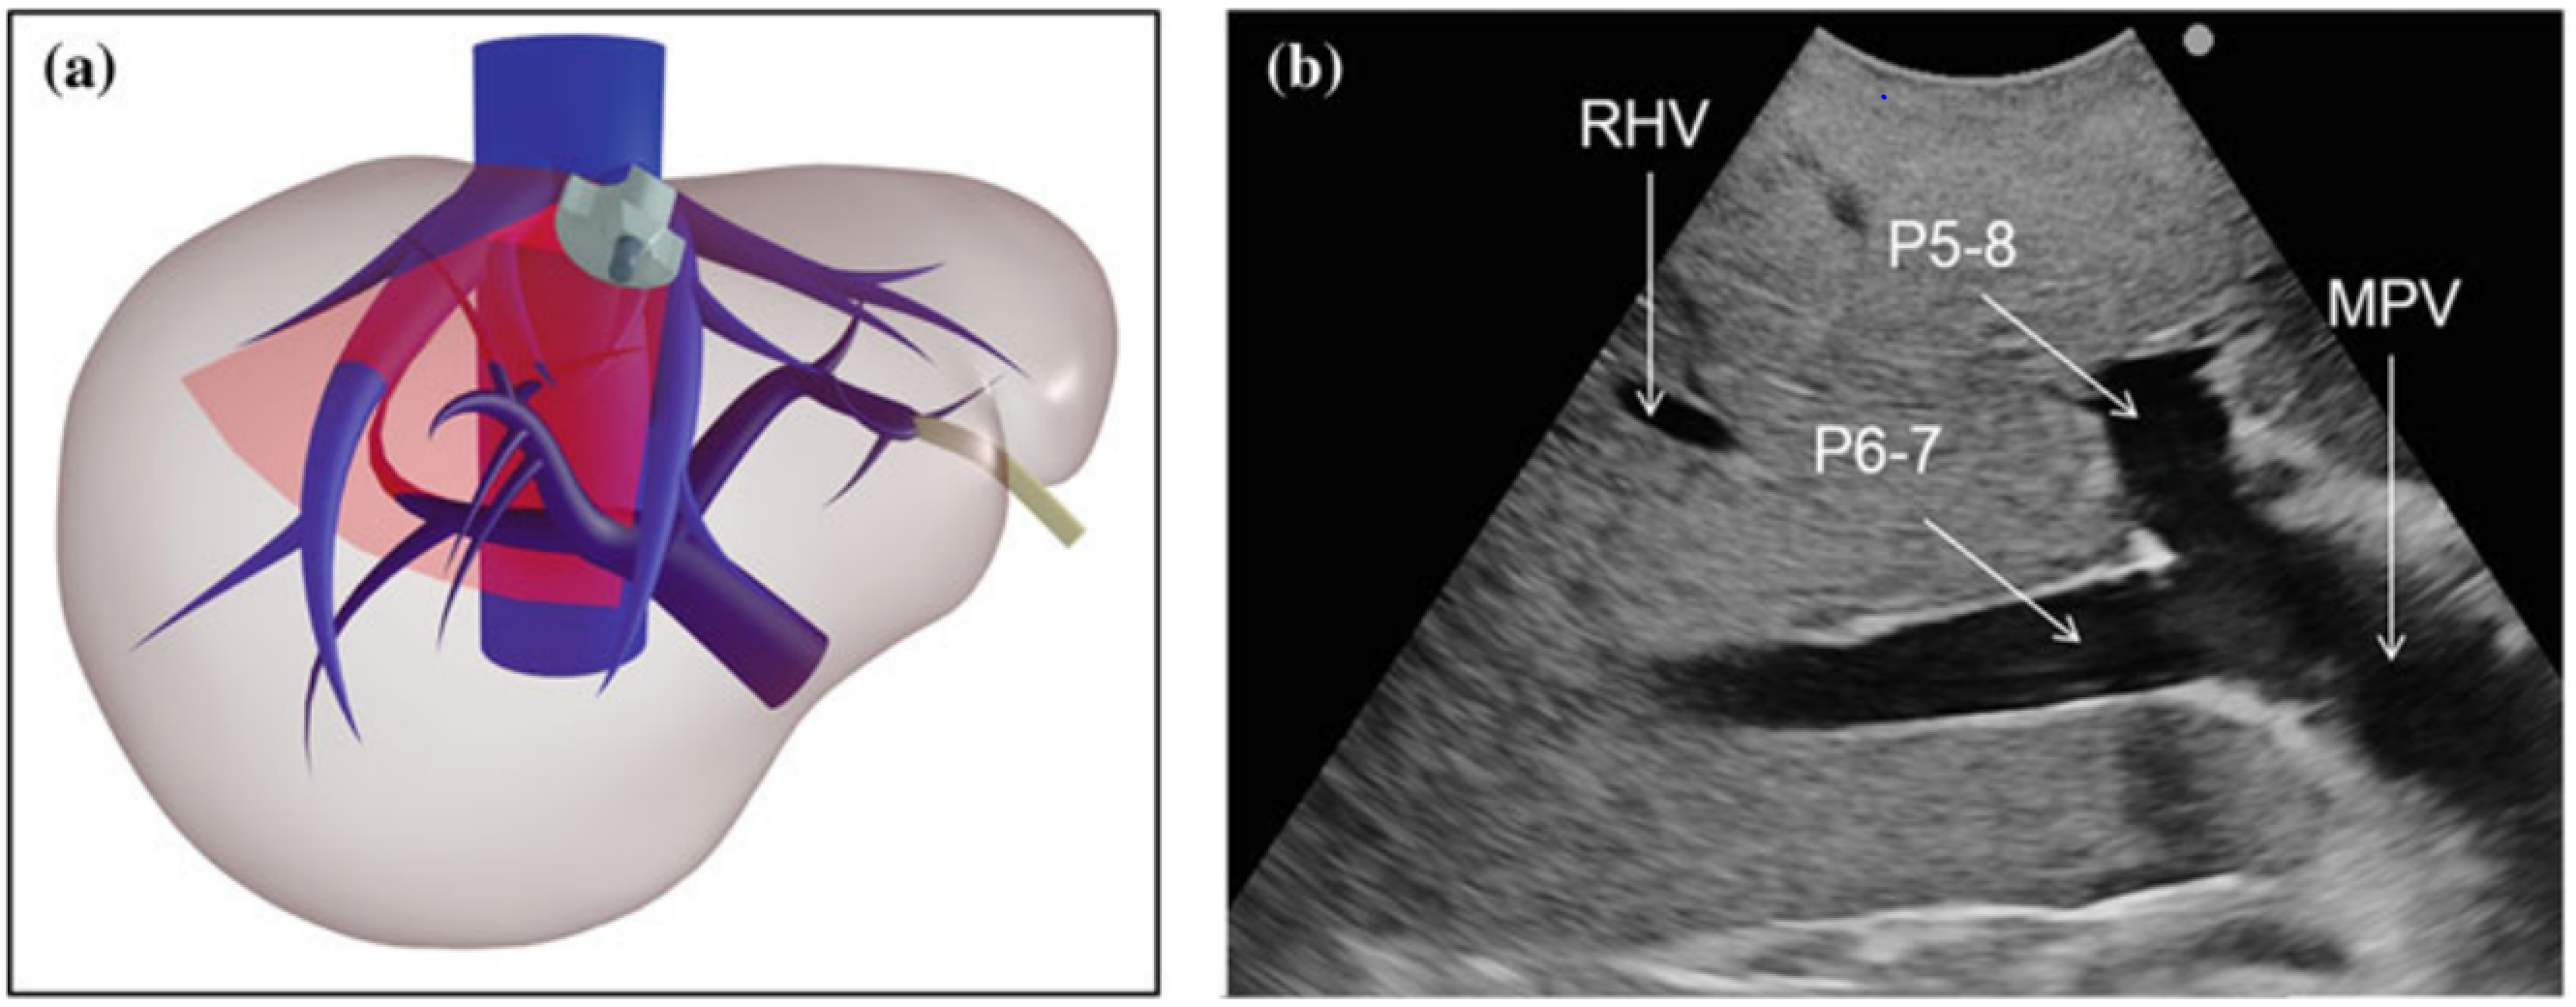
\includegraphics[width=\textwidth]{liverUS}
 \caption{ Left (a) ultrasound image plane in the liver. Right (b) intraoperative
   ultrasound image. One can see the right hepatic vein (RHV), the portal branch
   to segments 5 and 8 (P5-8) and the portal branch to segments 6 and 7 (P6-7) \cite{torzilli2014ultrasound}}
  \label{fig:liverUS}
\end{figure}

\section{Navigation for liver resections}
Navigation in liver surgeries is mostly done by registering the patient to a pre-operative 3D
computer tomography (CT) scan of the liver during the surgery. All surgical
instruments have trackable markers attached to them. A tracking camera sees
these markers and can differentiate the different instruments from their attached
markers. The achieved
navigation accuracy was 4.5 mm $\pm$3.6 mm averaged over nine surgeries \cite{peterhans2011navigation}.
Current research tries to compensate for deformations of the liver after the CT
scan to the actual shape \cite{clements2017deformation}
\cite{clements2015validation}. 

\subsection{Registration methods}
Different registration methods exist. Discrete landmarks, surface scans and
volumetric sonography scans are just a few of the approaches that can be
used to achieve precise alignment of the preoperative image data with the
surgical site \cite{banz2016intraoperative}.

\subsection{Tracking modalities}
To track surgical instruments and patient's anatomy (define the position and
orientation in real time) during naviagated surgery a tracking system is needed.
Tracking can be done by different technologies. The most used tracking
modality is optical tracking. 

\subsubsection{Optical tracking}
Optical tracking is the most used tracking modality in naviagated liver
surgeries. Passive markers (spherical, retro-reflective that reflect infrared
light) or active markers (infrared-emitting markers that are activated by an
electrical signal) \cite{wiles2004accuracy} are attached to the objects that
need to be tracked. A tracking camera is then emitting infrared light by illuminators
on the position sensor (only for passive markers). The position sensor
determines the position and orientation of the tracked instruments based on the
information it receives from those markers \cite{noauthor_polaris_nodate}.  

\section{Surface reconstruction}
A surface reconstruction's goal is to create a surface from sampling points. Two
main steps need to be processed. First, collecting the sample points. Second,
apply a reconstruction algorithm to the sampled points. There exist different
methods of collecting surface points
\cite{franca20053d}\cite{levoy2000digital}\cite{cui20113d}\cite{chu2002infrared}\cite{dou20153d}.
Optical (non-contact scan) scans are the most popular ones. Specialy laser based
scanners can scan very fast and with a precision in the order of micrometers. Also contact scans exist
\cite{pai2001scanning}. Contact scans can also be very precise (in the order of
micrometers).
The resulting sampling points lie on or near an unknown surface. A
reconstruction algorithm has now to reconstruct the surface from these points.
Again, a lot of reconstruction algorithms exist \cite{lim2014surface}. Only a
few articles were published in the
field of liver surface scanning \cite{maier2014comparative} \cite{thompson2015accuracy}. 



% \begin{itemize}
%   \item not tracked laproscopic one shot images stereo with registration
%   \item moved laproscopic tracked endoscope stereo with registration 
% \end{list}

% \cite{hoppe1992surface}

\endinput
%%% Local Variables:
%%% TeX-master: "MscThesis"
%%% End: